% ═══════════════════════════════════════════════════════════════════════════
%  DDF — préambule commun aux sept articles.  % ═══════════════════════════════════════════════════════════════════════════
%  DDF — préambule commun aux sept articles.  % ═══════════════════════════════════════════════════════════════════════════
%  DDF — préambule commun aux sept articles.  \input{ddf-common} en tête.
%  Définit : la mise en page, les macros, le bloc de série, la déclaration
%  d'usage d'outils, et le bloc de traçabilité.
% ═══════════════════════════════════════════════════════════════════════════
\documentclass[11pt,a4paper]{article}
\usepackage[margin=2.3cm]{geometry}
\usepackage{amsmath,amssymb,booktabs,hyperref,graphicx,xcolor}
\usepackage[expansion=false]{microtype}
\hypersetup{colorlinks=true,linkcolor=blue!45!black,citecolor=blue!45!black,urlcolor=blue!45!black}

% ---------- macros physiques ----------
\newcommand{\MPl}{M_{\rm Pl}}\newcommand{\Mred}{\bar M_{\rm Pl}}
\newcommand{\Mfive}{M_5}\newcommand{\MS}{M_S}\newcommand{\V}{\mathcal V}
\newcommand{\Neff}{N_{\rm eff}}\newcommand{\cb}{c_b}\newcommand{\ab}{\alpha_b}

% ---------- étiquettes épistémiques ----------
\newcommand{\Derived}{\textit{[Derived]}}
\newcommand{\Input}{\textit{[Input, natural]}}
\newcommand{\Posited}{\textit{[Posited]}}
\newcommand{\Candidate}{\textit{[Candidate]}}
\newcommand{\Open}{\textit{[Open, declared]}}
\newcommand{\Verified}{\textit{[Verified]}}

% ---------- bloc de série : \seriesdate{III}{The medium} ----------
\newcommand{\seriesdate}[2]{%
 \date{\small \textit{Cosmic Shadow Geometry} \\ \small Article #1 of VII
 \,\textperiodcentered\, #2 \,\textperiodcentered\, \today}}

% ---------- déclaration d'outils, identique dans les sept ----------
\newcommand{\toolsstatement}{%
\section*{Declaration on computational tools}
\addcontentsline{toc}{section}{Declaration on computational tools}
\small
This work was carried out by the author alone, without institutional affiliation.
\textbf{Large language models were used as computational and analytical assistants
throughout}: to write and debug the numerical scripts, to run the scans and
minimisations, to produce the figures, to check algebra and dimensional
consistency, to search and summarise the literature, and to audit drafts for
internal contradictions. Several distinct systems were used and cross-checked
against one another; no single system's output was accepted without an
independent numerical or analytical verification.

\textbf{The author is solely responsible for the physical hypotheses, the
interpretation of every result, the epistemic labels attached to each claim, and
the decision of what to publish and what to withdraw.} All quantitative
statements in this paper are reproduced by the scripts listed in the
traceability section; a reader who runs them obtains the numbers printed here
without needing any language model. Where an earlier draft contained an error
introduced by an unverified computation, it is recorded as a withdrawal rather
than silently removed.
\normalsize}

% ---------- bloc de traçabilité : \traceability{V}{...} ----------
\newcommand{\traceability}[2]{%
\section*{Data availability, traceability and reproducibility}
\addcontentsline{toc}{section}{Traceability}
\small
Every number, table and figure in this paper is regenerated by the scripts of
this article's folder. The complete repository ---sources, scripts, proof files,
figures and compiled documents for all seven articles--- is at
\url{https://github.com/HBoufourou}.

\textbf{Folder \texttt{article-#1/} contains:}
\begin{itemize}\itemsep2pt
\item \texttt{tex/} --- the \LaTeX\ source and the shared preamble \texttt{ddf-common.tex};
\item \texttt{scripts/} --- every computation, each runnable standalone with
      \texttt{python3 <name>.py} and printing its own verification verdict;
\item \texttt{proofs/} --- the JSON files carrying the certified values.
      \textbf{Any number absent from \texttt{proofs/} is not certified};
\item \texttt{data/} --- the CSV tables underlying the figures;
\item \texttt{figures/} --- the PNG files, regenerated by \texttt{scripts/figures.py};
\item \texttt{pdf/} --- the compiled article;
\item \texttt{VERIFICATION.txt} --- the output of the verification suite.
\end{itemize}
#2
\normalsize}
 en tête.
%  Définit : la mise en page, les macros, le bloc de série, la déclaration
%  d'usage d'outils, et le bloc de traçabilité.
% ═══════════════════════════════════════════════════════════════════════════
\documentclass[11pt,a4paper]{article}
\usepackage[margin=2.3cm]{geometry}
\usepackage{amsmath,amssymb,booktabs,hyperref,graphicx,xcolor}
\usepackage[expansion=false]{microtype}
\hypersetup{colorlinks=true,linkcolor=blue!45!black,citecolor=blue!45!black,urlcolor=blue!45!black}

% ---------- macros physiques ----------
\newcommand{\MPl}{M_{\rm Pl}}\newcommand{\Mred}{\bar M_{\rm Pl}}
\newcommand{\Mfive}{M_5}\newcommand{\MS}{M_S}\newcommand{\V}{\mathcal V}
\newcommand{\Neff}{N_{\rm eff}}\newcommand{\cb}{c_b}\newcommand{\ab}{\alpha_b}

% ---------- étiquettes épistémiques ----------
\newcommand{\Derived}{\textit{[Derived]}}
\newcommand{\Input}{\textit{[Input, natural]}}
\newcommand{\Posited}{\textit{[Posited]}}
\newcommand{\Candidate}{\textit{[Candidate]}}
\newcommand{\Open}{\textit{[Open, declared]}}
\newcommand{\Verified}{\textit{[Verified]}}

% ---------- bloc de série : \seriesdate{III}{The medium} ----------
\newcommand{\seriesdate}[2]{%
 \date{\small \textit{Cosmic Shadow Geometry} \\ \small Article #1 of VII
 \,\textperiodcentered\, #2 \,\textperiodcentered\, \today}}

% ---------- déclaration d'outils, identique dans les sept ----------
\newcommand{\toolsstatement}{%
\section*{Declaration on computational tools}
\addcontentsline{toc}{section}{Declaration on computational tools}
\small
This work was carried out by the author alone, without institutional affiliation.
\textbf{Large language models were used as computational and analytical assistants
throughout}: to write and debug the numerical scripts, to run the scans and
minimisations, to produce the figures, to check algebra and dimensional
consistency, to search and summarise the literature, and to audit drafts for
internal contradictions. Several distinct systems were used and cross-checked
against one another; no single system's output was accepted without an
independent numerical or analytical verification.

\textbf{The author is solely responsible for the physical hypotheses, the
interpretation of every result, the epistemic labels attached to each claim, and
the decision of what to publish and what to withdraw.} All quantitative
statements in this paper are reproduced by the scripts listed in the
traceability section; a reader who runs them obtains the numbers printed here
without needing any language model. Where an earlier draft contained an error
introduced by an unverified computation, it is recorded as a withdrawal rather
than silently removed.
\normalsize}

% ---------- bloc de traçabilité : \traceability{V}{...} ----------
\newcommand{\traceability}[2]{%
\section*{Data availability, traceability and reproducibility}
\addcontentsline{toc}{section}{Traceability}
\small
Every number, table and figure in this paper is regenerated by the scripts of
this article's folder. The complete repository ---sources, scripts, proof files,
figures and compiled documents for all seven articles--- is at
\url{https://github.com/HBoufourou}.

\textbf{Folder \texttt{article-#1/} contains:}
\begin{itemize}\itemsep2pt
\item \texttt{tex/} --- the \LaTeX\ source and the shared preamble \texttt{ddf-common.tex};
\item \texttt{scripts/} --- every computation, each runnable standalone with
      \texttt{python3 <name>.py} and printing its own verification verdict;
\item \texttt{proofs/} --- the JSON files carrying the certified values.
      \textbf{Any number absent from \texttt{proofs/} is not certified};
\item \texttt{data/} --- the CSV tables underlying the figures;
\item \texttt{figures/} --- the PNG files, regenerated by \texttt{scripts/figures.py};
\item \texttt{pdf/} --- the compiled article;
\item \texttt{VERIFICATION.txt} --- the output of the verification suite.
\end{itemize}
#2
\normalsize}
 en tête.
%  Définit : la mise en page, les macros, le bloc de série, la déclaration
%  d'usage d'outils, et le bloc de traçabilité.
% ═══════════════════════════════════════════════════════════════════════════
\documentclass[11pt,a4paper]{article}
\usepackage[margin=2.3cm]{geometry}
\usepackage{amsmath,amssymb,booktabs,hyperref,graphicx,xcolor}
\usepackage[expansion=false]{microtype}
\hypersetup{colorlinks=true,linkcolor=blue!45!black,citecolor=blue!45!black,urlcolor=blue!45!black}

% ---------- macros physiques ----------
\newcommand{\MPl}{M_{\rm Pl}}\newcommand{\Mred}{\bar M_{\rm Pl}}
\newcommand{\Mfive}{M_5}\newcommand{\MS}{M_S}\newcommand{\V}{\mathcal V}
\newcommand{\Neff}{N_{\rm eff}}\newcommand{\cb}{c_b}\newcommand{\ab}{\alpha_b}

% ---------- étiquettes épistémiques ----------
\newcommand{\Derived}{\textit{[Derived]}}
\newcommand{\Input}{\textit{[Input, natural]}}
\newcommand{\Posited}{\textit{[Posited]}}
\newcommand{\Candidate}{\textit{[Candidate]}}
\newcommand{\Open}{\textit{[Open, declared]}}
\newcommand{\Verified}{\textit{[Verified]}}

% ---------- bloc de série : \seriesdate{III}{The medium} ----------
\newcommand{\seriesdate}[2]{%
 \date{\small \textit{Cosmic Shadow Geometry} \\ \small Article #1 of VII
 \,\textperiodcentered\, #2 \,\textperiodcentered\, \today}}

% ---------- déclaration d'outils, identique dans les sept ----------
\newcommand{\toolsstatement}{%
\section*{Declaration on computational tools}
\addcontentsline{toc}{section}{Declaration on computational tools}
\small
This work was carried out by the author alone, without institutional affiliation.
\textbf{Large language models were used as computational and analytical assistants
throughout}: to write and debug the numerical scripts, to run the scans and
minimisations, to produce the figures, to check algebra and dimensional
consistency, to search and summarise the literature, and to audit drafts for
internal contradictions. Several distinct systems were used and cross-checked
against one another; no single system's output was accepted without an
independent numerical or analytical verification.

\textbf{The author is solely responsible for the physical hypotheses, the
interpretation of every result, the epistemic labels attached to each claim, and
the decision of what to publish and what to withdraw.} All quantitative
statements in this paper are reproduced by the scripts listed in the
traceability section; a reader who runs them obtains the numbers printed here
without needing any language model. Where an earlier draft contained an error
introduced by an unverified computation, it is recorded as a withdrawal rather
than silently removed.
\normalsize}

% ---------- bloc de traçabilité : \traceability{V}{...} ----------
\newcommand{\traceability}[2]{%
\section*{Data availability, traceability and reproducibility}
\addcontentsline{toc}{section}{Traceability}
\small
Every number, table and figure in this paper is regenerated by the scripts of
this article's folder. The complete repository ---sources, scripts, proof files,
figures and compiled documents for all seven articles--- is at
\url{https://github.com/HBoufourou}.

\textbf{Folder \texttt{article-#1/} contains:}
\begin{itemize}\itemsep2pt
\item \texttt{tex/} --- the \LaTeX\ source and the shared preamble \texttt{ddf-common.tex};
\item \texttt{scripts/} --- every computation, each runnable standalone with
      \texttt{python3 <name>.py} and printing its own verification verdict;
\item \texttt{proofs/} --- the JSON files carrying the certified values.
      \textbf{Any number absent from \texttt{proofs/} is not certified};
\item \texttt{data/} --- the CSV tables underlying the figures;
\item \texttt{figures/} --- the PNG files, regenerated by \texttt{scripts/figures.py};
\item \texttt{pdf/} --- the compiled article;
\item \texttt{VERIFICATION.txt} --- the output of the verification suite.
\end{itemize}
#2
\normalsize}

\graphicspath{{figures/}{../figures/}}
\title{\textbf{The Dark Dimension Framework I:\\ The stage --- a mesoscopic dark dimension and its brane}}
\author{Hicham Boufourou\\ \small\textit{Independent Researcher, Brussels, Belgium}\\ \small\texttt{hicham.boufourou@hotmail.com}}
\seriesdate{I}{The stage}
\begin{document}\maketitle
\begin{abstract}
\noindent This is the first of five articles presenting the Dark Dimension Framework in its final form: a five-dimensional framework in which a single mesoscopic extra dimension --- an interval of $R=8.2~\mu$m --- carries gravity and one dark scalar, while the Standard Model lives on a thin brane at one boundary. This article builds the stage. The radius is fixed by a conditional Casimir calibration against the dark-energy density, $\Lambda=C/R^{4}$: the calibration explains the \emph{relation} between the size of the dimension and the acceleration of the universe, and is explicit about what it does not explain --- the absolute value, which is the cosmological-constant problem, inherited and declared. The brane is modelled as a field-theoretic thin core in the lineage of domain-wall localisation: for a wall whose parameters sit at a single scale $m_\chi$, the tension and the localisation width obey $T^{1/4}=L_{g}^{-1}=m_\chi$ at order unity, so the framework's two TeV requirement windows overlap because they are one scale. Gravity alone spreads into the interval; its dilution is why it is weak, and its Kaluza--Klein tower changes the force law below $R$ with a parameter-free strength $\alpha=8/3$ --- the framework's principal laboratory test, currently a factor $\sim65$ below torsion-balance sensitivity at $8~\mu$m and moving into reach. The radion is treated honestly: its mass is an order estimate ($m_{r}R/\hslash c=0.37$, not computed), so the framework predicts a \emph{window}, 5--40~meV, not a line; its Planckian inertia locks the dark-energy equation of state to $|1+w|\lesssim10^{-61}$ and forbids, by one theorem read twice, both a first-order transition and decompactification. The baryon--bulk interaction is written as a covariant boundary operator coupling the bulk scalar to the trace of the localised stress tensor; the reduction gives the amplitude $\alpha_{b}=c_{b}\sqrt{2w_{1}}$ with $c_{b}$ an order-unity ultraviolet vertex --- the thin-core computation shows the boundary overlap equals unity to twenty-six decimal places, so $c_{b}$ is an input, natural and declared, whose numerical weight $w_{1}$ is computed in Article II. Budgets close the stage: the dark sector must be cold ($T_{d}/T_{\gamma}<0.60$ today, $<0.40$ under CMB-S4), the brane portal is bounded through the Airy tail at the far edge, and the stellar-cooling judge sharpened by others still passes. The article ends, as every article of this series does, by stating how it dies.
\end{abstract}

\section{Purpose, rules, and the shape of the series}
the Dark Dimension Framework proposes that dark matter, dark energy and the anomalous rotation of galaxies are three behaviours of one structure: a fifth spatial dimension of micron size, closed by two boundaries, inhabited by gravity and a single dark scalar field, with all of ordinary physics confined to a thin brane at one wall. The framework was developed, audited and stress-tested over an extended programme whose traceability dossiers accompany this series; the present four articles are its final, self-contained statement. Article I (this one) builds the stage: the geometry, the brane, gravity in the bulk, the radion, the covariant baryon--bulk vertex, and the budgets. Article II derives the confining well and the discrete tower of the dark scalar from brane sources, and closes the amplitude accounting. Article III presents the medium: the two roles of the dark field --- particulate reservoir and coherent mediator --- its cosmological history, its galactic response, and where that response switches off. Article IV states the structure of the whole: one TeV scale and its gravitationally transmitted meV shadow, the convergence that supports it, and the complete map of what is derived, what is input, and what only data can decide. This framework is a dark dimension in the sense of Montero, Vafa and Valenzuela; the name records its central structure, the shadow relation of Article~IV, under which the entire millielectronvolt sector is the gravitational shadow of one TeV scale. A fifth article, cited throughout as the \emph{companion}, examines whether this geometry admits an ultraviolet completion in Type~I$'$ string theory; it is a companion, not a foundation, and nothing in Articles~I--IV depends on it.

Three rules govern every page. First, \emph{labels}: every quantitative statement carries one of [Derived] (follows from the framework's inputs with no freedom), [Posited] (a choice, declared), [Input, natural] (a constant not derivable at the effective-theory level, with its naturalness stated), [Candidate] (a structural relation supported at order of magnitude, not yet a derivation), [Open, declared] (a genuine unknown, kept visible), or [S-3] (the cosmological-constant class: inherited, not created here, and not claimed solved). Second, \emph{reproducibility}: every number in the text is produced by a script in the article's dossier; nothing is quoted from memory. Third, \emph{mortality}: each article closes with the specific measurements that would kill it. A framework that cannot die is not physics; this one states its executioners by name.

\section{The interval and the Casimir calibration}
\subsection{Geometry}
Spacetime is five-dimensional with signature $(-,+,+,+,+)$: one time, four space. The fifth dimension is compactified on the orbifold $S^{1}/\mathbb{Z}_{2}$, equivalent to an interval $y\in[0,\pi R]$ bounded by two four-dimensional walls. Our wall sits at $y=0$; the far wall, required by the geometry, carries nothing in the minimal framework and is predicted to be empty. [In the Type~I$'$ realisation examined in the companion, local tadpole cancellation places a non-chiral hidden gauge sector on that wall; the prediction survives in its own terms --- no Standard-Model matter --- and the hidden sector falls under the same $\Delta N_{\rm eff}$ budget declared in \S8. See Appendix~C.] The compactification relates the fundamental and effective gravitational scales by volume,
\begin{equation}
\MPl^{2}=\Mfive^{3}\,(\pi R),
\label{eq:volume}
\end{equation}
the volume being the physical length of the interval --- the orbifold identifies the two halves of the covering circle, so the space gravity spreads into is $\pi R$, not $2\pi R$. With the radius fixed below, $\Mfive=3.6\times10^{8}$~GeV; translated into the species-scale convention of the dark-dimension literature, $\Lambda_{\rm QG}=(\MPl^{2}m_{\rm KK})^{1/3}\approx1.5\times10^{9}$~GeV with the unreduced Planck mass --- inside that programme's $10^{9}$--$10^{10}$~GeV band, so the two bookkeepings describe the same physics. Gravity is not weak, it is diluted, and its true scale is mesoscopic in energy just as the dimension is mesoscopic in length. [Derived, given $R$]

\subsection{The calibration}
A bounded vacuum is never empty: between two walls the zero-point energy of the confined fields depends on the separation --- the Casimir effect, measured in the laboratory since 1997. Applied to the interval, the residual vacuum energy scales as
\begin{equation}
\Lambda=\frac{C}{R^{4}},
\label{eq:casimir}
\end{equation}
with $C$ an order-unity coefficient set by the light bulk field content. Equating this to the observed dark-energy density $\rho_{\Lambda}=(2.25~\mathrm{meV})^{4}$ fixes
\begin{equation}
R=8.2~\mu\mathrm{m},\qquad \pi R=25.8~\mu\mathrm{m}.
\end{equation}
This is the framework's founding calibration, and its epistemic status must be stated with care. What it explains is a \emph{relation}: if a micron-scale dimension exists, the acceleration of the universe measures its size, and conversely every laboratory probe of gravity below $40~\mu$m is a probe of dark energy. What it does not explain is the \emph{value}: why the vacuum energy is $(2.25~\mathrm{meV})^{4}$ rather than the $\sim(10^{18}~\mathrm{GeV})^{4}$ of naive counting is the cosmological-constant problem, and this framework inherits it whole. The honest accounting is that the framework reduces the problem from a conspiracy among unwritten terms to a single written line --- Eq.~(\ref{eq:casimir}) with its bare contribution cancelled --- which is its best available form, and no more. [Calibration: Derived as a relation; the value: S-3, declared]

The coincidence that launched the mesoscopic-dimension programme in the wider literature --- that $\rho_{\Lambda}^{1/4}$ sits at the millimetre--micron gravitational frontier --- is here promoted to the framework's central identification, and Article IV will show that the same millielectronvolt scale is reached a second, independent way, as the gravitational shadow of a TeV scale.

\emph{What fixes what.} The framework's dependency chain is short and worth displaying: $\rho_{\Lambda}$ (measured) $\to$ $R$ (Eq.~\ref{eq:casimir}) $\to$ $\Mfive$ (Eq.~\ref{eq:volume}) and the position of every laboratory window; the wall scale $m_\chi$ (TeV) is fixed independently by the requirements of \S3 and Article II; the meV scale of the bulk sector will be reached a second way in Article IV. Two measured numbers --- the dark-energy density and, prospectively, one TeV-scale quantity --- anchor the entire geometry. Everything else in this article is either a pure number ($\alpha=8/3$, the Airy ratios of Article II) or a declared window.

\section{The brane as a thin core at one scale}
\subsection{The wall, not a postulate}
The brane is not an axiom but an object: a field-theoretic domain wall, in the lineage that predates string-theoretic branes by more than a decade \cite{RS83}. A five-dimensional scalar $\chi$ with a symmetry-breaking potential forms a kink; four-dimensional fermions arise as zero modes trapped on it \cite{RS83}, and gauge fields are localised by the standard confinement mechanism \cite{DS97}, which this series treats as the known solution to the classical difficulty of brane-worlds and does not rebuild. [Posited mechanism, standard]

\subsection{One scale, two windows}
A wall has two basic attributes: a tension $T$ (energy per unit three-volume) and a thickness $L_{g}$ (the localisation width of the fields it carries). For a five-dimensional kink these are
\begin{equation}
T\sim\frac{m_\chi^{3}}{\lambda_\chi},\qquad L_{g}^{-1}\sim m_\chi ,
\end{equation}
with $m_\chi$ the wall mass scale and $\lambda_\chi$ its self-coupling of dimension $\mathrm{GeV}^{-1}$. For a wall whose parameters sit at a \emph{single} scale --- $\lambda_\chi\sim1/m_\chi$, the most natural choice, meaning the wall is strongly coupled at its own mass --- the ratio collapses:
\begin{equation}
\frac{T^{1/4}}{L_{g}^{-1}}=\left(\frac{1}{\lambda_\chi m_\chi}\right)^{1/4}=1\quad\text{at order unity.}
\label{eq:onescale}
\end{equation}
The framework's requirement analysis produces two independent TeV windows: the tension window $T^{1/4}\in2$--$13$~TeV, from demanding that the brane's gravitational pull bind one to four levels of the dark tower (the derivation lives in Article II), and the thickness window $L_{g}^{-1}\in1$--$10$~TeV from localisation-width consistency. Equation~(\ref{eq:onescale}) says these overlap \emph{because they are the same scale}: what looked like a numerical coincidence between two requirements is the signature of a one-scale wall. [Derived, $\mathcal{O}(1)$] Nothing of the Standard Model propagates into the bulk --- not the photon, not the nucleon, not you; only gravity and the dark scalar of Article II do. The corridor is dark because it is empty of everything that shines.

\begin{figure}[t]
\centering
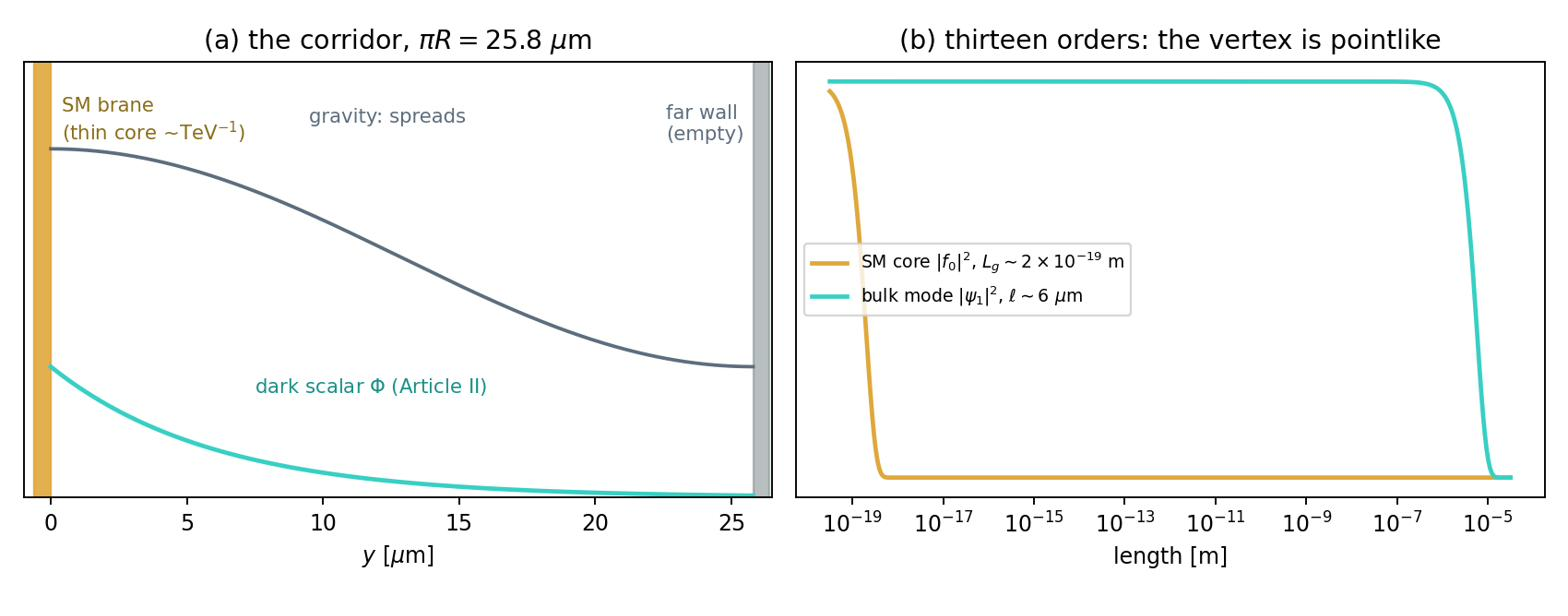
\includegraphics[width=0.98\textwidth]{fig1_stage.png}
\caption{The stage. Left: the interval $[0,\pi R]$ with the Standard Model confined to a thin core (width $\sim\mathrm{TeV}^{-1}=2\times10^{-19}$~m) at $y=0$, the far wall empty, and only gravity and the dark scalar spreading across the $25.8~\mu$m corridor. Right: the thirteen orders of magnitude between the core width and the bulk wavefunctions (Article II) --- the reason the boundary vertex of \S6 is pointlike to twenty-six decimal places. [Schematic; scales from \texttt{core\_scale.py}]}
\label{fig:stage}
\end{figure}

\section{Gravity in the corridor: dilution, the $8/3$ law, and two laboratory judges}
\subsection{Why gravity is weak, and where it stops being Newtonian}
A refrigerator magnet lifts a paper clip against the gravity of the entire Earth. In this framework the disproportion has a geometric cause: among the interactions, gravity alone spreads into the corridor, and Eq.~(\ref{eq:volume}) is the accounting of its dilution. The same statement has a sharp short-distance consequence. The graviton acquires a Kaluza--Klein tower of massive modes; at separations approaching $R$ their exchange modifies the inverse-square law,
\begin{equation}
V(r)=-\frac{G m_{1}m_{2}}{r}\left[1+\alpha\, e^{-r/R}\right],\qquad \alpha=\frac{8}{3},
\end{equation}
where $\alpha=8/3$ is the parity-projected tower strength for one flat extra dimension \cite{KS00} --- a pure number, independent of every open input of the framework. [Derived] The prediction is therefore uncommonly rigid: a Yukawa correction of strength exactly $8/3$ at range exactly $8.2~\mu$m. Calibrating on the published torsion-balance exclusion of $\alpha=1$ for ranges above $38.6~\mu$m at $52~\mu$m minimum separation \cite{Lee20}, the predicted signal lies a factor $\sim65$ below current sensitivity at $R=8.2~\mu$m ($3.1$ at $15~\mu$m). This is the framework's principal test: not a hint to be fitted, but a fixed point to be hit or missed. [Derived; the judge]

\subsection{The laboratory analogue}
The mathematics that will organise Article II --- a quantum field bound against a wall by a linear potential, with Airy-function levels --- is not exotic: it is laboratory physics. Ultracold neutrons bouncing on a mirror in the Earth's field occupy exactly such gravitational quantum states, with the Airy energy unit $\varepsilon\approx0.6$~peV and a first level near $1.4$~peV, resolved experimentally since 2002 \cite{Nesv02}. The quantum bouncer plays two roles here: it is the verified analogue of the dark tower one dimension higher, and it is a judge in its own right --- any new micron-range force couples to the bouncing neutron, and the continued agreement of its level spectrum with Newtonian gravity independently constrains the framework's short-range sector. [Analogue and judge]

\subsection{The exclusion map}
The short-range sector of the framework is not one prediction but a spectrum, and it is worth laying the whole map on the table (Fig.~\ref{fig:ranges}). The graviton tower contributes at ranges $R/n$ with parity-projected, brane-weighted strengths --- the leading fixed point $\alpha=8/3$ at $8.2~\mu$m, with higher modes at $4.1$, $2.7~\mu$m\ldots{} carrying weights that fall as $1/b_{n}$; all strengths are pure numbers. The radion contributes a single Yukawa of order-unity strength somewhere in the 5--40~$\mu$m window --- the one entry whose position is an order estimate, and whose lower edge the data already set. The dark scalar of Article II contributes \emph{nothing}: its source field couples to the brane's tension, not to matter, and its own tower is gravitationally weighted --- the corridor's matter content leaves the short-range landscape clean. The map's value is its rigidity: every filled feature has a fixed strength, so any deviation found at the wrong $(\alpha,\lambda)$ point falsifies the framework as surely as no deviation at the right one. [Derived map; one windowed entry]

\section{The radion: stiffness, the window, and the double no-go}
\subsection{An order estimate, declared as such}
The size of the corridor can breathe: its fluctuation is a four-dimensional scalar, the radion --- the $h_{55}$ component of the five-dimensional graviton, the quantum of the geometry's own deformation. Its mass is where this framework practises the honesty it preaches. The stabilising potential is not derived from the residual $\Lambda$ --- it cannot be: a modulus stabilised at the dark-energy scale would weigh $\sim10^{-33}$~eV, and the stiffness actually required, $V_{\rm stab}\sim m_{r}^{2}\MPl^{2}$, sits sixty-one orders above the residual vacuum energy. That gap \emph{is} the cosmological-constant problem again, met from a second direction, and it is declared, not hidden. What the framework asserts is the natural expectation for a compactification modulus, $m_{r}\sim\mathcal{O}(1)/R$; numerically $m_{r}R/\hslash c=0.37$, a coefficient of order unity that is \emph{not computed}, and whose computation would require a concrete stabilisation mechanism --- a Goldberger--Wise scalar with TeV-scale boundary values, or an equivalent --- which this framework does not yet contain. The consequence is drawn without flinching:
\begin{equation}
m_{r}\in5\text{--}40~\mathrm{meV}\quad\Longleftrightarrow\quad \text{range}\;\hslash c/m_{r}\in5\text{--}40~\mu\mathrm{m}:
\end{equation}
the radion is a \emph{window}, not a line --- and the window is an order estimate, not a prediction: its factor-eight width reflects the absence of a computed coefficient, and a stabilisation mechanism would narrow it to a line. The lower edge is already experimental: the same torsion-balance exclusion quoted above forbids an order-unity radion Yukawa beyond $38.6~\mu$m, hence $m_{r}>5.11$~meV --- the laboratory bound is presently sharper than the theory, and the framework acknowledges the division of labour: the data set the floor, the theory sets the window. Inverting the required stiffness gives $V_{\rm stab}^{1/4}=\sqrt{m_{r}\MPl}\approx3.5$--$10$~TeV; a Casimir-only stabilisation is excluded by its own curvature (it would leave $m_{r}\sim10^{-32}$~eV, thirty orders below the fifth-force floor), so the stiffness must come from TeV physics on the wall --- a thread Article IV picks up and ties. [Order estimate, declared; window Derived from it]

What would convert the window into a line is a concrete stabilisation mechanism. The capacitor of Article II cannot serve: its contribution to the radion mass falls twenty-eight orders short of the required stiffness, and the two sectors remain independent. A Goldberger--Wise scalar with TeV-scale boundary values would work in principle, and Article IV's shadow relation suggests that the required stiffness is exactly what a TeV-scale wall would provide --- but the construction of that mechanism is the task of the framework's second stage, not of this article. Until then, the window stands as the honest limit of what the geometry alone can assert: an order estimate, labelled as such, with its width reflecting the absence of the mechanism rather than the uncertainty of the theory.

\subsection{One theorem, two protections}
The radion's kinetic term is Planckian --- it is a piece of the metric --- and this single fact protects the universe twice. First, its vacuum cannot decay by bubble nucleation: the instanton action scales as $S\sim\MPl^{2}/m_{r}\sim10^{45}$, so the corridor undergoes no first-order transition, ever. Second, the same action forbids decompactification: the minimum at $8.2~\mu$m is local --- $R\to\infty$ is always a runaway direction --- but the barrier is crossed at rate $e^{-10^{45}}$, a lifetime of $10^{10^{45}}$~seconds. The width of the world is frozen. The same stiffness locks the dark-energy equation of state, $\delta R/R\sim\rho/(m_{r}^{2}\MPl^{2})$ giving $|1+w|\lesssim10^{-61}$ --- a Hooke's law for the geometry, and a prediction DESI-class surveys test for free. And it closes a door worth closing explicitly: no laboratory source can bend the geometry (deforming $R$ by one part per million would require $\sim5\times10^{11}$ times nuclear density), so the framework contains no exploitable warp channel; the navigable universe and the habitable universe are the same universe, and it chose stability. [Derived; robust to the $m_{r}$ uncertainty, which enters only as $1/m_{r}$]

\subsection{The third lock: the corridor never rolled far}
A modulus that settles leaves a relic. The classical roll of $R$ towards its minimum deposits a coherent oscillation of the radion field, which redshifts as non-relativistic matter --- the cosmological moduli problem, met here in its mildest form and stated as a constraint rather than a signal. Oscillation begins when $H\simeq m_{r}$, that is at
\begin{equation}
T_{\rm osc}=\sqrt{\frac{m_{r}\MPl}{1.66\sqrt{g_{*}}}}\;\simeq\;4~\mathrm{TeV}\quad (2\text{--}5~\mathrm{TeV}\ \text{across the window}),
\end{equation}
and the relic density that follows from an initial displacement $\rho_{i}$ is $\Omega_{r}h^{2}\simeq3.6\times10^{12}\,(\rho_{i}/\MPl)^{2}$ at $m_{r}=24$~meV. A Planckian displacement would therefore overclose the universe by thirteen orders of magnitude, and requiring $\Omega_{r}h^{2}\leq0.12$ gives
\begin{equation}
\frac{\delta R}{R}\Big|_{\rm initial}\;\lesssim\;10^{-7}.
\end{equation}
The fifth dimension must have been born within about one part in ten million of its final width. Three things follow, and the framework declares all three. It is a genuine constraint on initial conditions --- a fine-tuning, of the class that afflicts every light modulus, and not resolved here; the standard escapes (an inflationary scale below $m_{r}$, so that the modulus is never displaced, or entropy production after $T_{\rm osc}$) are available but neither is derived by this framework, so the constraint is filed [Open, declared] rather than dismissed. It \emph{completes the radion's mortality clause}: the corridor does not tunnel, does not unwind (\S5.2), and did not roll far --- the geometry has been still since before the electroweak era, and its stillness is now a number rather than an assumption. And it carries a structural remark that Article IV will collect: since the shadow relation makes $m_{r}\sim M_{S}^{2}/\MPl$, the oscillation temperature is $T_{\rm osc}\sim\sqrt{m_{r}\MPl}\sim M_{S}$ up to $\mathcal{O}(1)$ --- \textbf{the radion begins to oscillate at the scale of the wall that cast it}. The shadow returns to its source. [Derived constraint; the fine-tuning: Open, declared]

\section{The covariant brane vertex}
The bulk scalar $\Phi$ of Article II must talk to ordinary matter, or the medium of Article III would have no galactic voice. The interaction is written once, covariantly, as a boundary operator:
\begin{equation}
S_{\rm int}=-\frac{c_{b}}{\Mfive^{3/2}}\int d^{5}x\,\sqrt{-g_{5}}\;\delta(y-y_{0})\;\Phi\; g_{\mu\nu}T_{b}^{\mu\nu},
\label{eq:vertex}
\end{equation}
the trace of the localised baryonic stress tensor. Because $T_{b}^{\mu\nu}$ is covariantly conserved on the brane, the coupling respects four-dimensional diffeomorphism and gauge invariance and introduces no gradient instabilities. Kaluza--Klein reduction on the ground profile of $\Phi$, with the boundary weight $w_{1}\equiv\pi R\,|\psi_{1}(y_{0})|^{2}$ and the volume calibration Eq.~(\ref{eq:volume}), yields the effective four-dimensional amplitude
\begin{equation}
\alpha_{b}\;=\;c_{b}\,\sqrt{2w_{1}},
\label{eq:alpha}
\end{equation}
an identity verified symbolically in the dossier. Two statements complete the vertex, one structural, one honest. Structural: the thin core of \S3 makes the $\delta$-function exact for all practical purposes --- the overlap correction is $(L_{g}/\ell)^{2}\sim10^{-27}$, with $\ell$ the micron-scale bulk wavelength of Article II --- so Eq.~(\ref{eq:alpha}) receives no form-factor ambiguity. Honest: by the same token $c_{b}$ \emph{is} the ultraviolet vertex itself, and its numerical value is not derivable at the effective-field-theory level; it is an [Input, natural], expected of order unity --- the companion derives the tree-level coupling \emph{vector} of a Type~I$'$ embedding and an upper bound on this constant, but not its value, so the label stands unchanged (Appendix~C) ---, and Article II will show that with $w_{1}=5.5$ the galactic phenomenology indeed requires $c_{b}$ of order unity --- the accounting closes with nothing forced. [Vertex: Derived at the operator level; $c_{b}$: Input, natural]

\begin{figure}[t]
\centering
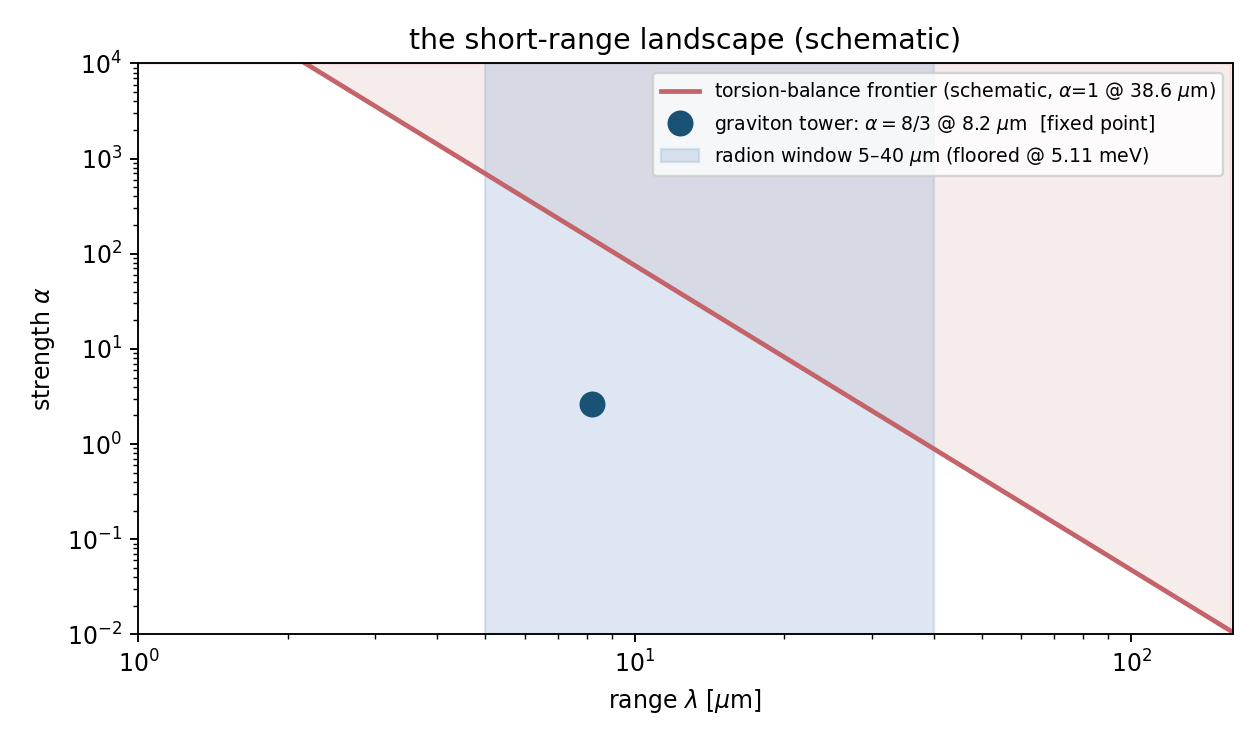
\includegraphics[width=0.86\textwidth]{fig2_ranges.png}
\caption{The short-range landscape of the framework in the $(\alpha,\lambda)$ plane, schematic. The fixed point of the graviton tower ($\alpha=8/3$ at $\lambda=8.2~\mu$m, filled marker) sits a factor $\sim65$ below the current torsion-balance frontier (solid line, calibrated on the published exclusion of $\alpha=1$ beyond $38.6~\mu$m); the radion is a window, 5--40~$\mu$m (band), floored at $5.11$~meV by the same data; the source field of Article II leaves no trace here at all. [Schematic; numbers from \texttt{core\_scale.py} and \cite{Lee20}]}
\label{fig:ranges}
\end{figure}

\section{Budgets: what the bulk is allowed to contain}
The stage would collapse if the corridor's contents disturbed precision cosmology or astrophysics; three budgets say it does not, and each is a standing judge.

\emph{Radiation budget.} Every light bulk field contributes to the effective neutrino number. The dark sector of this framework is populated cold and dilute (Article III), never thermalised with the plasma; the requirement reads $\Delta N_{\rm eff}=g\,(4/7)(T_{d}/T_{\gamma})^{4}<0.3$ today, satisfied for the framework's light bulk content (four effective degrees of freedom) provided $T_{d}/T_{\gamma}<0.60$ --- and tightening to $<0.40$ under a CMB-S4-class bound of $0.06$. The budget is not a loophole but a forecast: each future field added to the bulk must be colder than the last, and the next CMB generation adjudicates.

\emph{And the bound is in fact a prediction.} That the sector is never thermalised is not an assumption but a consequence of the vertex itself. The operator $(c_{b}/\Mfive^{3/2})\Phi\,g_{\mu\nu}T^{\mu\nu}$ is of dimension five, so the production rate scales as $\Gamma\sim T^{5}/M^{4}$ with $M=\MPl/c_{b}$, against $H\sim T^{2}/\MPl$; equilibrium would require
\begin{equation}
T_{\rm eq}=\MPl\,c_{b}^{-4/3},
\end{equation}
which exceeds the Planck mass for every $c_{b}$ below $2.1$ --- that is, across the entire range this framework admits. \textbf{The dark sector cannot reach thermal contact with the plasma at any epoch}, so $T_{d}$ is not a free parameter bounded from above: it is whatever produced the sector. Misalignment produces it cold, and a cold component contributes as matter, not as radiation. What remains is the unavoidable gravitational production through the same vertex, of relative size $c_{b}^{2}(T_{\rm reh}/\MPl)^{3}$: at $T_{\rm reh}=10^{16}$~GeV this gives $\Delta N_{\rm eff}\sim3\times10^{-8}$, and at the settling scale of Article~III it is smaller than $10^{-40}$.

\textbf{The framework therefore predicts $\Delta N_{\rm eff}\simeq0$, not merely $<0.3$}, and this is the sharper statement: a bound cannot be violated from below, but a prediction of zero can. A CMB-S4-class detection of $\Delta N_{\rm eff}\simeq0.06$ would not tighten this framework --- it would refute it, unless the excess is attributed to the hidden sector discussed in Appendix~C. [Derived]

\emph{Portal budget.} The brane portal --- mixing between bulk and Standard-Model states --- is doubly suppressed: by the gravitational-strength vertex and, for any state leaking to the far wall, by the Airy tail across the corridor, $e^{-(2/3)(\pi R/\ell)^{3/2}}$, giving relative weights $0.25$ at one bound level down to $4\times10^{-6}$ at four. The framework's portal angle is bounded at $\theta<4\times10^{-16}$, which subsumes the SN1987A cooling constraint with room to spare. The gravitational realisation makes the sector darker, at the declared price that no portal signal is expected. [Derived]

\emph{Stellar budget.} Kaluza--Klein graviton emission cools stars; for a single extra dimension the recent dedicated analysis \cite{Hardy} finds bounds weaker than the laboratory frontier --- the judge has been sharpened by others, and the framework still passes. [External judge, passed]

\begin{table}[h]
\centering\small
\begin{tabular}{lll}
\toprule
\textbf{Quantity} & \textbf{Value} & \textbf{Status}\\
\midrule
Radius $R$ & $8.2~\mu$m & Calibrated on $\rho_{\Lambda}$ [relation Derived; value S-3]\\
Fundamental scale $\Mfive$ & $3.6\times10^{8}$~GeV & [Derived from $R$]\\
Tower strength $\alpha$ & $8/3$ at $8.2~\mu$m & [Derived; parameter-free]\\
Wall scale $m_\chi=T^{1/4}=L_{g}^{-1}$ & $\sim$1--10~TeV & [Derived $\mathcal{O}(1)$; windows unified]\\
Radion mass $m_{r}$ & 5--40~meV window & [Order estimate, declared; floor: data]\\
Equation of state & $|1+w|\lesssim10^{-61}$ & [Derived]\\
Vertex amplitude $\alpha_{b}$ & $c_{b}\sqrt{2w_{1}}$ & [Derived; $c_{b}$ Input-natural]\\
Dark temperature & $T_{d}/T_{\gamma}<0.60$ & [Derived requirement]\\
Portal angle & $\theta<4\times10^{-16}$ & [Derived]\\
\bottomrule
\end{tabular}
\caption{The stage in one table. Every entry is reproduced by the dossier scripts.}
\end{table}

\section{How this article dies}
The stage is falsifiable on its own, before the medium ever enters. (i) \emph{The balance:} a torsion-balance campaign reaching Yukawa strength $8/3$ at $8.2~\mu$m and finding Newton kills the framework outright --- there is no parameter to move; conversely a deviation of the wrong strength or the wrong range kills it just as dead. (ii) \emph{The window:} closure of the 5--40~$\mu$m band without a radion signal removes the stabilised-geometry sector and, through Article IV, the framework's structural capstone. (iii) \emph{The bouncer:} a shift in the neutron's gravitational levels attributable to a micron-range force of the wrong size contradicts the same sector. (iv) \emph{The budgets:} a CMB-S4 measurement of $\Delta N_{\rm eff}$ above budget, or any confirmed portal signal, breaks the cold-and-dark accounting. (v) \emph{The radion window:} if a stabilisation mechanism is constructed and predicts a radion mass outside the 5--40~meV window, or if the window closes without a radion signal, the geometry's breathing mode is falsified --- the window is an order estimate; a line outside it, or an empty window, kills it. (vi) \emph{The relic}: a cosmology that requires an initial radion displacement above $10^{-7}\MPl$ --- or a measurement of dark-matter substructure demanding a meV relic scalar of exactly this stiffness --- collides with the third lock. Article II now builds what lives inside this stage: the well, the tower, and the closed amplitude.


% ═══════════════════════════════════════════════════════════════════════════
%  APPENDICE DE LIAISON — identique dans les sept articles.
%  % ═══════════════════════════════════════════════════════════════════════════
%  APPENDICE DE LIAISON — identique dans les sept articles.
%  % ═══════════════════════════════════════════════════════════════════════════
%  APPENDICE DE LIAISON — identique dans les sept articles.
%  \input{appendix-where} juste avant \begin{thebibliography} ou la biblio.
%  Il répond à : qui vit où, et qu'est-ce que la série a changé en cours de route.
% ═══════════════════════════════════════════════════════════════════════════
\section*{Appendix: which sector lives where, and what changed}
\addcontentsline{toc}{section}{Appendix: which sector lives where}

The series was written over several months and \textbf{two of its assignments moved}.
A reader who meets the articles out of order is owed an explicit map rather than an
inference, so it is given here, identically in all seven papers.

\subsection*{A.1 The three locations}
The geometry has three places where physics can sit: the \emph{brane} at $y=0$,
the \emph{bulk} of the $8.2\,\mu$m interval, and the \emph{far wall} at $y=\pi R$.
\begin{center}\small
\begin{tabular}{llll}\toprule
sector & lives on & carried by & established in\\\midrule
ordinary matter & \textbf{brane} & thin core, Standard Model & I\\
gravity, radion, graviton & \textbf{bulk} & five-dimensional fields & I\\
the mediator $\Phi$ and its tower & \textbf{bulk} & Airy states of the $|y|$ well & II\\
the galactic response & \textbf{bulk} $\to$ brane & $\Phi$ exchange between baryons & III\\
dark matter & \textbf{see A.2} & --- & III, revisited in VI\\
dark energy & \textbf{see A.3} & --- & III, revisited in VI\\
hidden gauge sector & \textbf{far wall} & eight D8 and one O8 & V\\\bottomrule
\end{tabular}
\end{center}

\subsection*{A.2 Dark matter: the reservoir, and what the wall reading adds}
Articles~I--IV place dark matter in the \emph{bulk}: the excited states of the Airy
tower, populated cold at birth, collisionless, carrying at least $98.6\%$ of the dark
sector's density. That assignment does the work in three places. It makes structure
formation identical to cold dark matter at linear order. It answers the Bullet Cluster
by mass budget alone --- cluster masses are cluster masses, and the lensing tracks the
reservoir, which is why the lensing--dynamics difficulty of purely modified dynamics is
not inherited. And it fixes the radiation budget of Article~I.

Article~VI proposes a different reading: dark matter as the ordinary matter of the six
other regions of the same wall, seen through the bulk, giving
$\Omega_{\rm DM}/\Omega_b=N_{\rm regions}-1=6$ against an observed $5.31$.
\textbf{These are not the same statement, and we do not pretend otherwise.}

What they share is everything the phenomenology uses: in both readings the dark
component is cold, collisionless, and carries the mass, so lensing, the Bullet Cluster
and linear structure formation are unaffected. What differs is the \emph{constituent}:
quanta of $\Phi$ in the first, baryons of other regions in the second.
\textbf{The two are compatible if the tower reservoir is not required to be the whole
of the dark matter} --- and Article~III's own argument only requires it to dominate the
budget, not to be exhaustive. \Open

\subsection*{A.3 Dark energy: a bulk scalar, then a brane curvature}
Articles~I--IV treat $\Phi$ as the dark-energy candidate --- a bulk scalar engine. That
attempt \emph{failed by forty orders of magnitude}: a four-dimensional scalar cannot
reach $2.4$~meV from a $10^{-13}$~eV engine scale. The failure is recorded, not hidden.

Article~VI relocates dark energy \emph{to the brane}, as the extrinsic curvature of the
D8 wall in the cosmological bulk, $\Lambda_4=\varepsilon^2(1/R)^4$ with
$\varepsilon\simeq10^{-2}$. The mechanism supplies $(1/R)^4$ outright and leaves a gap
of $10^4$ rather than $10^{40}$. \textbf{$\Phi$ is correspondingly demoted from
dark-energy candidate to dark-sector mediator}, which is the role Articles~II and III
already gave it in every equation they actually use. \Candidate, declared tuning.

\subsection*{A.4 The radial acceleration relation, and what makes galaxies turn}
The relation is the one place where brane and bulk are \emph{both} indispensable, and
where nothing has moved since Article~III.

Baryons sit on the brane. They source $\Phi$, which propagates in the bulk with mass
$m_\Phi=24$~meV and hence Compton range $8.2\,\mu$m --- microscopic, so no fifth force
acts between laboratory bodies. What acts at galactic scale is not the free field but
the \emph{medium}: the coherent component of the dark sector responds to the baryonic
distribution, and that response, read back on the brane, is the extra acceleration.
The response saturates, which is why it produces a relation --- an acceleration scale
$g_\dagger$ --- rather than a rescaling of Newton's constant.

Three consequences, all in Article~III and unchanged:
\begin{itemize}\itemsep2pt
\item the response couples to the trace $T^\mu_{\ \mu}$, hence to mass and not to
      composition; the universality is bounded on 171 SPARC galaxies;
\item the response is carried by at most $1.4\%$ of the dark sector, the coherent part,
      so it never competes with the reservoir in the mass budget --- \textbf{galaxies
      turn because of the medium, they weigh because of the reservoir};
\item the response \emph{dies} in weak field, which is the ultra-diffuse galaxy test,
      and it dies in a decoherence bubble around the Sun, which is why Cassini is
      satisfied identically rather than by tuning.
\end{itemize}
\textbf{Neither relocation of A.2 or A.3 touches this.} The galactic response was never
assigned to the dark-energy sector, and it is not the reservoir either; it is the third
role, and it is the one the framework was built to explain.

\subsection*{A.5 What a reader should carry between articles}
Articles~I--IV stand on their own evidence and are not modified by V--VII: no result of
theirs is derived from the string embedding, and the embedding cannot promote any of
their labels. What V--VII add is an ultraviolet origin for one constant, a candidate
geometry, and two consequences of that geometry. What they \emph{change} is recorded
above and nowhere else: two relocations, both declared, neither retroactive.
 juste avant \begin{thebibliography} ou la biblio.
%  Il répond à : qui vit où, et qu'est-ce que la série a changé en cours de route.
% ═══════════════════════════════════════════════════════════════════════════
\section*{Appendix: which sector lives where, and what changed}
\addcontentsline{toc}{section}{Appendix: which sector lives where}

The series was written over several months and \textbf{two of its assignments moved}.
A reader who meets the articles out of order is owed an explicit map rather than an
inference, so it is given here, identically in all seven papers.

\subsection*{A.1 The three locations}
The geometry has three places where physics can sit: the \emph{brane} at $y=0$,
the \emph{bulk} of the $8.2\,\mu$m interval, and the \emph{far wall} at $y=\pi R$.
\begin{center}\small
\begin{tabular}{llll}\toprule
sector & lives on & carried by & established in\\\midrule
ordinary matter & \textbf{brane} & thin core, Standard Model & I\\
gravity, radion, graviton & \textbf{bulk} & five-dimensional fields & I\\
the mediator $\Phi$ and its tower & \textbf{bulk} & Airy states of the $|y|$ well & II\\
the galactic response & \textbf{bulk} $\to$ brane & $\Phi$ exchange between baryons & III\\
dark matter & \textbf{see A.2} & --- & III, revisited in VI\\
dark energy & \textbf{see A.3} & --- & III, revisited in VI\\
hidden gauge sector & \textbf{far wall} & eight D8 and one O8 & V\\\bottomrule
\end{tabular}
\end{center}

\subsection*{A.2 Dark matter: the reservoir, and what the wall reading adds}
Articles~I--IV place dark matter in the \emph{bulk}: the excited states of the Airy
tower, populated cold at birth, collisionless, carrying at least $98.6\%$ of the dark
sector's density. That assignment does the work in three places. It makes structure
formation identical to cold dark matter at linear order. It answers the Bullet Cluster
by mass budget alone --- cluster masses are cluster masses, and the lensing tracks the
reservoir, which is why the lensing--dynamics difficulty of purely modified dynamics is
not inherited. And it fixes the radiation budget of Article~I.

Article~VI proposes a different reading: dark matter as the ordinary matter of the six
other regions of the same wall, seen through the bulk, giving
$\Omega_{\rm DM}/\Omega_b=N_{\rm regions}-1=6$ against an observed $5.31$.
\textbf{These are not the same statement, and we do not pretend otherwise.}

What they share is everything the phenomenology uses: in both readings the dark
component is cold, collisionless, and carries the mass, so lensing, the Bullet Cluster
and linear structure formation are unaffected. What differs is the \emph{constituent}:
quanta of $\Phi$ in the first, baryons of other regions in the second.
\textbf{The two are compatible if the tower reservoir is not required to be the whole
of the dark matter} --- and Article~III's own argument only requires it to dominate the
budget, not to be exhaustive. \Open

\subsection*{A.3 Dark energy: a bulk scalar, then a brane curvature}
Articles~I--IV treat $\Phi$ as the dark-energy candidate --- a bulk scalar engine. That
attempt \emph{failed by forty orders of magnitude}: a four-dimensional scalar cannot
reach $2.4$~meV from a $10^{-13}$~eV engine scale. The failure is recorded, not hidden.

Article~VI relocates dark energy \emph{to the brane}, as the extrinsic curvature of the
D8 wall in the cosmological bulk, $\Lambda_4=\varepsilon^2(1/R)^4$ with
$\varepsilon\simeq10^{-2}$. The mechanism supplies $(1/R)^4$ outright and leaves a gap
of $10^4$ rather than $10^{40}$. \textbf{$\Phi$ is correspondingly demoted from
dark-energy candidate to dark-sector mediator}, which is the role Articles~II and III
already gave it in every equation they actually use. \Candidate, declared tuning.

\subsection*{A.4 The radial acceleration relation, and what makes galaxies turn}
The relation is the one place where brane and bulk are \emph{both} indispensable, and
where nothing has moved since Article~III.

Baryons sit on the brane. They source $\Phi$, which propagates in the bulk with mass
$m_\Phi=24$~meV and hence Compton range $8.2\,\mu$m --- microscopic, so no fifth force
acts between laboratory bodies. What acts at galactic scale is not the free field but
the \emph{medium}: the coherent component of the dark sector responds to the baryonic
distribution, and that response, read back on the brane, is the extra acceleration.
The response saturates, which is why it produces a relation --- an acceleration scale
$g_\dagger$ --- rather than a rescaling of Newton's constant.

Three consequences, all in Article~III and unchanged:
\begin{itemize}\itemsep2pt
\item the response couples to the trace $T^\mu_{\ \mu}$, hence to mass and not to
      composition; the universality is bounded on 171 SPARC galaxies;
\item the response is carried by at most $1.4\%$ of the dark sector, the coherent part,
      so it never competes with the reservoir in the mass budget --- \textbf{galaxies
      turn because of the medium, they weigh because of the reservoir};
\item the response \emph{dies} in weak field, which is the ultra-diffuse galaxy test,
      and it dies in a decoherence bubble around the Sun, which is why Cassini is
      satisfied identically rather than by tuning.
\end{itemize}
\textbf{Neither relocation of A.2 or A.3 touches this.} The galactic response was never
assigned to the dark-energy sector, and it is not the reservoir either; it is the third
role, and it is the one the framework was built to explain.

\subsection*{A.5 What a reader should carry between articles}
Articles~I--IV stand on their own evidence and are not modified by V--VII: no result of
theirs is derived from the string embedding, and the embedding cannot promote any of
their labels. What V--VII add is an ultraviolet origin for one constant, a candidate
geometry, and two consequences of that geometry. What they \emph{change} is recorded
above and nowhere else: two relocations, both declared, neither retroactive.
 juste avant \begin{thebibliography} ou la biblio.
%  Il répond à : qui vit où, et qu'est-ce que la série a changé en cours de route.
% ═══════════════════════════════════════════════════════════════════════════
\section*{Appendix: which sector lives where, and what changed}
\addcontentsline{toc}{section}{Appendix: which sector lives where}

The series was written over several months and \textbf{two of its assignments moved}.
A reader who meets the articles out of order is owed an explicit map rather than an
inference, so it is given here, identically in all seven papers.

\subsection*{A.1 The three locations}
The geometry has three places where physics can sit: the \emph{brane} at $y=0$,
the \emph{bulk} of the $8.2\,\mu$m interval, and the \emph{far wall} at $y=\pi R$.
\begin{center}\small
\begin{tabular}{llll}\toprule
sector & lives on & carried by & established in\\\midrule
ordinary matter & \textbf{brane} & thin core, Standard Model & I\\
gravity, radion, graviton & \textbf{bulk} & five-dimensional fields & I\\
the mediator $\Phi$ and its tower & \textbf{bulk} & Airy states of the $|y|$ well & II\\
the galactic response & \textbf{bulk} $\to$ brane & $\Phi$ exchange between baryons & III\\
dark matter & \textbf{see A.2} & --- & III, revisited in VI\\
dark energy & \textbf{see A.3} & --- & III, revisited in VI\\
hidden gauge sector & \textbf{far wall} & eight D8 and one O8 & V\\\bottomrule
\end{tabular}
\end{center}

\subsection*{A.2 Dark matter: the reservoir, and what the wall reading adds}
Articles~I--IV place dark matter in the \emph{bulk}: the excited states of the Airy
tower, populated cold at birth, collisionless, carrying at least $98.6\%$ of the dark
sector's density. That assignment does the work in three places. It makes structure
formation identical to cold dark matter at linear order. It answers the Bullet Cluster
by mass budget alone --- cluster masses are cluster masses, and the lensing tracks the
reservoir, which is why the lensing--dynamics difficulty of purely modified dynamics is
not inherited. And it fixes the radiation budget of Article~I.

Article~VI proposes a different reading: dark matter as the ordinary matter of the six
other regions of the same wall, seen through the bulk, giving
$\Omega_{\rm DM}/\Omega_b=N_{\rm regions}-1=6$ against an observed $5.31$.
\textbf{These are not the same statement, and we do not pretend otherwise.}

What they share is everything the phenomenology uses: in both readings the dark
component is cold, collisionless, and carries the mass, so lensing, the Bullet Cluster
and linear structure formation are unaffected. What differs is the \emph{constituent}:
quanta of $\Phi$ in the first, baryons of other regions in the second.
\textbf{The two are compatible if the tower reservoir is not required to be the whole
of the dark matter} --- and Article~III's own argument only requires it to dominate the
budget, not to be exhaustive. \Open

\subsection*{A.3 Dark energy: a bulk scalar, then a brane curvature}
Articles~I--IV treat $\Phi$ as the dark-energy candidate --- a bulk scalar engine. That
attempt \emph{failed by forty orders of magnitude}: a four-dimensional scalar cannot
reach $2.4$~meV from a $10^{-13}$~eV engine scale. The failure is recorded, not hidden.

Article~VI relocates dark energy \emph{to the brane}, as the extrinsic curvature of the
D8 wall in the cosmological bulk, $\Lambda_4=\varepsilon^2(1/R)^4$ with
$\varepsilon\simeq10^{-2}$. The mechanism supplies $(1/R)^4$ outright and leaves a gap
of $10^4$ rather than $10^{40}$. \textbf{$\Phi$ is correspondingly demoted from
dark-energy candidate to dark-sector mediator}, which is the role Articles~II and III
already gave it in every equation they actually use. \Candidate, declared tuning.

\subsection*{A.4 The radial acceleration relation, and what makes galaxies turn}
The relation is the one place where brane and bulk are \emph{both} indispensable, and
where nothing has moved since Article~III.

Baryons sit on the brane. They source $\Phi$, which propagates in the bulk with mass
$m_\Phi=24$~meV and hence Compton range $8.2\,\mu$m --- microscopic, so no fifth force
acts between laboratory bodies. What acts at galactic scale is not the free field but
the \emph{medium}: the coherent component of the dark sector responds to the baryonic
distribution, and that response, read back on the brane, is the extra acceleration.
The response saturates, which is why it produces a relation --- an acceleration scale
$g_\dagger$ --- rather than a rescaling of Newton's constant.

Three consequences, all in Article~III and unchanged:
\begin{itemize}\itemsep2pt
\item the response couples to the trace $T^\mu_{\ \mu}$, hence to mass and not to
      composition; the universality is bounded on 171 SPARC galaxies;
\item the response is carried by at most $1.4\%$ of the dark sector, the coherent part,
      so it never competes with the reservoir in the mass budget --- \textbf{galaxies
      turn because of the medium, they weigh because of the reservoir};
\item the response \emph{dies} in weak field, which is the ultra-diffuse galaxy test,
      and it dies in a decoherence bubble around the Sun, which is why Cassini is
      satisfied identically rather than by tuning.
\end{itemize}
\textbf{Neither relocation of A.2 or A.3 touches this.} The galactic response was never
assigned to the dark-energy sector, and it is not the reservoir either; it is the third
role, and it is the one the framework was built to explain.

\subsection*{A.5 What a reader should carry between articles}
Articles~I--IV stand on their own evidence and are not modified by V--VII: no result of
theirs is derived from the string embedding, and the embedding cannot promote any of
their labels. What V--VII add is an ultraviolet origin for one constant, a candidate
geometry, and two consequences of that geometry. What they \emph{change} is recorded
above and nowhere else: two relocations, both declared, neither retroactive.

\toolsstatement
\traceability{1}{The radiation budget of \S8 and the Casimir, radion and spectrum computations are produced by the scripts of \texttt{scripts/}.}
\bibliographystyle{unsrt}\bibliography{ddf-refs}

\section*{Appendix C: what the companion does, and does not, provide}
\addcontentsline{toc}{section}{Appendix C}
\label{app:companion}

A fifth article --- \emph{The Dark Dimension Framework from Type~I$'$ strings}, cited here as the companion --- asks whether the geometry of Articles~I--IV admits an ultraviolet completion. It is deposited together with this series so that a reader who asks \emph{where does this constant come from?} has somewhere to look. Three statements govern how it may be used.

\paragraph{It is a companion, not a foundation.} Every result, label and executioner of Articles~I--IV is established at the effective-theory level and stands or falls on its own evidence. If the companion's embedding is refuted tomorrow, nothing in this article changes. The converse also holds: the companion cannot promote a label here, and none of its findings has been used to do so.

\paragraph{What it establishes.} The companion shows that the framework's boundary conditions ($J_{0}+J_{\pi}=0$) are literally the Ramond--Ramond tadpole cancellation of a Type~I$'$ orientifold; it derives, at tree level, the coupling vector through which brane tension reaches the bulk scalar, obtaining three integer norm identities and an upper bound on the boundary constant, $c_{b}\leq\sqrt{255/56}=2.13$; it establishes two autonomous negative results (five independent moduli-pinning mechanisms fail, and massive type~IIA is incompatible with a mesoscopic interval); and it exhibits one explicit candidate vacuum that passes every computable test. For the present article the relevant items are two: the boundary vertex of \S6 is the object the companion computes, and the far wall of \S2 acquires a hidden, non-chiral gauge sector whose radiation budget is the one already declared in \S8.

\paragraph{What it does not establish.} It does not derive the value of $c_{b}$. That value depends on the mixing angle of the light modulus, which in turn depends on string-loop coefficients that are not computable for a general Calabi--Yau manifold --- a frontier of that field, not of this construction. The companion therefore closes with a conditional statement, not a number. \textbf{Accordingly, no label in Articles~I--IV is altered by it}: what was [Input, natural] remains so, and what was [Open, declared] remains open. A further consequence is recorded here rather than in the body: the companion's flat subspace is two-dimensional, so the moduli sector carries \emph{two} light scalars whose towers differ by four parts in $10^{8}$ and are therefore experimentally indistinguishable. No result of this series is falsified by this --- the phenomenology does not separate them --- but the radiation budget of \S8 would be counted with two towers rather than one, tightening its bound from $T_{d}/T_{\gamma}<0.60$ to $<0.57$. More consequentially, the radiation budget changes target. Because the tower cannot thermalise (\S8) it predicts $\Delta N_{\rm eff}\simeq0$; the hidden gauge sector that tadpole cancellation places on the far wall is then the only candidate source of a non-zero value. \textbf{The budget of \S8 therefore ceases to constrain the effective theory, which predicts zero, and begins to constrain the embedding.} The value quoted in \S8 is the one this article derives from its own content and stands unchanged; the tightening is a consequence of the embedding, and belongs to it.

\end{document}